\section{TTGO-Lora-Funk-ESP32 }
Der TTGO-Lora-Funk-ESP32 ist ein leistungsstarker Mikrocontroller, der speziell für die Verwendung in der drahtlosen Datenübertragung entwickelt wurde. 
Er basiert auf dem ESP32-Chip von Espressif-Systems und verfügt über ein integriertes LoRa-Funkmodul, das eine drahtlose Kommunikation über große Entfernungen ermöglicht.
Die Verwendung des ESP32-Chips bietet dem TTGO-Lora-Funk-ESP32 eine hohe Rechenleistung und Speicherkapazität. 
Der Chip verfügt über einen Dual-Core-Prozessor mit einer Taktrate von bis zu 240 MHz, der eine schnelle Datenverarbeitung ermöglicht. 
Darüber hinaus bietet der Chip bis zu 4 MB Flash-Speicher und bis zu 520 KB SRAM, was ausreichend Platz für die Speicherung von Programmcode und Daten bietet.
Das integrierte LoRa-Funkmodul ermöglicht die drahtlose Übertragung von Daten über große Entfernungen. Es unterstützt eine Übertragungsgeschwindigkeit von bis zu 300 kbps und eine Reichweite von bis zu 10 km in ländlichen Gebieten und bis zu 2 km in städtischen Gebieten da dort die Signale von den Gebäuden geschwächt werden. Dies macht den TTGO-Lora-Funk-ESP32 ideal für Anwendungen, die eine drahtlose Kommunikation über große Entfernungen erfordern, wie beispielsweise die Überwachung von Umgebungsbedingungen in der Landwirtschaft oder die Übertragung von Daten in Smart-City-Anwendungen. Im Zuge dieser Diplomarbeit kam diese Funktion zur Verwendung um die von den Sensoren gelesenen Daten an einen zweiten ESP-32 mit identer Ausstattung zu senden und von dort für das Flutter Frontend bereit zu stellen. 
Der TTGO-Lora-Funk-ESP32 ist auch mit einer Vielzahl von Schnittstellen ausgestattet, die eine einfache Integration in verschiedene Anwendungen ermöglichen. Er verfügt über einen Micro-USB-Anschluss für die Stromversorgung und Programmierung, sowie über einen JST-XH-Anschluss um eine externe Batterie anzuschließen. Darüber hinaus verfügt der Mikrocontroller über GPIO-Pins, I2C-, SPI- und UART-Schnittstellen, die eine einfache Integration mit Sensoren, Displays und anderen Geräten ermöglichen.
Der TTGO-Lora-Funk-ESP32 ist auch mit einer Vielzahl von Open-Source-Entwicklertools und Bibliotheken kompatibel.  Unter anderem kann das Framework Arduino IDE verwendet werden, um den Mikrocontroller zu programmieren, und es gibt eine Vielzahl von Bibliotheken für LoRa-Funk und andere Funktionen, die von der Community entwickelt wurden. Dies erleichtert die Entwicklung von Anwendungen mit dem TTGO-Lora-Funk-ESP32 und reduziert die Entwicklungszeit.
Darüber hinaus bietet der TTGO-Lora-Funk-ESP32 eine kosteneffektive Lösung für die drahtlose Datenübertragung. Im Vergleich zu anderen drahtlosen Übertragungstechnologien wie Mobilfunk oder Wi-Fi ist LoRa-Funk eine kosteneffektive Alternative, die auch in ländlichen Gebieten oder in Gebieten mit schlechter Netzabdeckung funktioniert.
Eine weitere Stärke des TTGO-Lora-Funk-ESP32 ist seine Energieeffizienz. Der ESP32-Chip unterstützt verschiedene Energiesparmodi und bietet einen integrierten Stromsparmodus, der die Energieaufnahme des Mikrocontrollers reduziert, wenn er nicht aktiv ist. Dies ist besonders nützlich in batteriebetriebenen Anwendungen, da es die Lebensdauer der Batterie verlängert.
Ein weiterer Vorteil des TTGO-Lora-Funk-ESP32 ist seine Unterstützung durch eine aktive Community von Entwicklern. Es gibt eine Vielzahl von Foren und Online-Communities, die sich auf die Entwicklung von Anwendungen mit dem TTGO-Lora-Funk-ESP32 spezialisiert haben. Dies macht es einfacher, Unterstützung und Hilfe zu finden, wenn man bei der Entwicklung von Anwendungen auf Probleme stößt.
Da der TTGO-Lora-Funk-ESP32 ein leistungsstarker und vielseitiger Mikrocontroller ist, der für die drahtlose Datenübertragung entwickelt wurde eine hohe Rechenleistung besitzt, dazu aber noch kosten- und energieeffizient ist, fiel die Entscheidung bei dieser Arbeit auf ihn.

\begin{figure}[b]
    \centering
    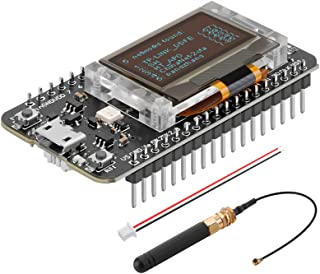
\includegraphics[width=0.5\textwidth]{./pics/ttgoLoraOled.jpg}
    \caption{ESP32-TTGO-LoRa-Oled}
    \label{fig:TTGO-ESP32}
  \end{figure}

\newpage
\section{ESP32-Chip:}


\textbf{}
\begin{itemize}
    \item Der ESP32 unterstützt bis zu 4 × 16 MB externen Speicher.
    \item Man kann den internen Takt (8 MHz) oder einen
    externen Quarztakt mit üblicherweise 160 MHz nutzen. 
    Wenn man den Prozessor zurück setzt übernimmt er auch das System-Timing.
    \item Hall-Sensor: Kann für die Messung von Magnetfeldschwankungen genutzt werden.
    \item Ein interner Temperatursensor mit einem Messbereich von –40 bis 125 Grad ist ebenfalls vorhanden.
    Die analogen Messwerte werden wie bei dem Hall-Sensor
    von einem Analog-Digital-Wandler digitalisiert. 
    In neueren Modellen ist kein Temperatur Sensor mehr verbaut.
    \item Es sind 34 GPIOs (universelle Ein- und Ausgänge) vorhanden. 
    Verwendet werden diese für Ein-und Ausgabe analoger und digitaler Signale. 
    Die Pins sind mehrfach belegt. 
    Mit internen Pull-down und Pull-up-Widerständen können definierte Zustände herbeigeführt werden.
    \item Der ESP32 kann Signale von bis zu zehn unterschiedlichen TouchSensoren verarbeiten. 
    \item Der ESP32 Unterstützt Bluetooth als auch W-Lan im 2.4-GHz Bereich und kann diese 
    Empfangen und Senden. 
    \item Es wird Bluetooth 4.2 und Bluetooth low-energy unterstützt.
    \item Der ESP32 hat vier 64-Bit-Universaltimer. Diese kann man via Software steuern.
    \item Es gibt Watchdog-Timer. Man unterscheidet zwischen Main-Watchdog-Timern und RTC-Watchdog-Timern. 
    Auslösen kann man hiermit einen CPU-Reset , ein Core-Reset oder ein Interrupt.
    \item  12-Bit-A/D-Wandler (Analog-Digital-Wandler) mit 18 Kanälen 
    \item  8-Bit-DAC (Digital-Analog-Wandler)
    \item SPI-Schnittstellen (SPI1, HSPI and VSPI) mit Master- oder Slave-Modus
    \item Es werden zwei I2C-Bus-Schnittstellen vorgehalten, die im Master- oder SlaveModus betrieben werden können.
    \item Pulsweitenmodulation (PWM) um Geräte wie Motoren, elektrische Heizungen oder Ähnliches zu steuern. 
    
\end{itemize}

\section{LoRa-Funk Modul:}
LoRa (Long Range) ist eine drahtlose Übertragungstechnologie, die speziell für den Einsatz in IoT (Internet of Things) Anwendungen entwickelt wurde. 
Das LoRa-Funk-Modul ist ein elektronisches Bauteil, das die LoRa-Technologie integriert und es Geräten ermöglicht, Daten über große Entfernungen drahtlos zu übertragen. 
Das LoRa-Funk-Modul arbeitet auf der Basis von Funkfrequenzen im ISM-Band (Industrial, Scientific and Medical Band) von 868 MHz oder 915 MHz. 
Diese Frequenzen ermöglichen eine Übertragung von Daten über Entfernungen von bis zu 10 Kilometern, was die LoRa-Technologie ideal für den Einsatz in Anwendungen wie Smart-Cities, Landwirtschaft oder Industrie macht. 
Ein weiterer Vorteil des LoRa-Funk-Moduls ist seine geringe Stromaufnahme. Die LoRa-Technologie nutzt ein Spread-Spectrum-Verfahren, das eine hohe Signalstärke bei einer geringen Bandbreite ermöglicht. 
Dadurch kann das Modul mit einer geringen Sendeleistung arbeiten, was wiederum zu einer längeren Lebensdauer der Batterie führt. 
Das LoRa-Funk-Modul ist auch sehr zuverlässig. 
Die Technologie nutzt „Forward Error Correction“ (FEC), um Datenübertragungsfehler zu erkennen und zu korrigieren. 
Dadurch wird eine zuverlässige Übertragung von Daten über große Entfernungen ermöglicht, auch in Umgebungen mit schlechter Netzabdeckung. 
Das LoRa-Funk-Modul ist auch sehr einfach zu integrieren. Es ist kompatibel mit einer Vielzahl von Mikrocontrollern und kann über verschiedene Schnittstellen wie UART oder SPI angeschlossen werden. 
Darüber hinaus gibt es eine Vielzahl von Bibliotheken und Entwicklertools, die von der Community entwickelt wurden, um die Integration mit verschiedenen Plattformen und Anwendungen zu erleichtern. 
\newline 
Zusammenfassend ist das LoRa-Funk-Modul eine leistungsfähige und zuverlässige drahtlose Übertragungstechnologie, die speziell für den Einsatz in IoT-Anwendungen entwickelt wurde und deshalb perfekt für dieses Projekt geignet ist.


\newpage
\section{Verwendete Sensoren:}
\subsection*{TemperaturSensor:}
Der DS18B20 ist ein digitaler Temperatursensor, der von der Firma Maxim Integrated entwickelt wurde. Es handelt sich um einen 1-Wire-Sensor, der eine hohe Genauigkeit und Zuverlässigkeit bietet und in einer Vielzahl von Anwendungen eingesetzt wird.
Der DS18B20 besteht aus einem temperaturabhängigen Sensor, einem Analog-Digital-Converter (ADC) und einer seriellen Schnittstelle. Der Sensor ist in einem wasserdichten Edelstahlgehäuse untergebracht, das ihn vor äußeren Einflüssen wie Feuchtigkeit, Staub und Schmutz schützt. Der ADC wandelt das analoge Ausgangssignal des Sensors in ein digitales Signal um, das über die serielle Schnittstelle übertragen wird.
Der DS18B20 bietet eine hohe Genauigkeit mit einer Auflösung von bis zu 12 Bit und einer Genauigkeit von ±0,5°C im Temperaturbereich von -10°C bis +85°C. Der Sensor bietet auch eine schnelle Reaktionszeit mit einer Konvertierungsrate von bis zu 750 ms pro Konvertierung.
Ein weiterer Vorteil des DS18B20 ist seine einfache Verbindung mit einem Mikrocontroller oder einem Computer. Der Sensor verwendet nur einen Daten-Pin und eine Spannungsversorgung und kann daher leicht in ein System integriert werden. Der 1-Wire-Bus, der vom Sensor verwendet wird, ermöglicht auch die Verbindung mehrerer Sensoren an denselben Daten-Pin, was eine effiziente und kostengünstige Möglichkeit bietet, die Temperatur in verschiedenen Teilen eines Systems zu überwachen.
Der DS18B20 bietet auch eine programmierbare Auflösung, die es ermöglicht, die Genauigkeit des Sensors an die spezifischen Anforderungen einer Anwendung anzupassen. Entwickler können die Auflösung des Sensors auf 9, 10, 11 oder 12 Bit programmieren, um eine höhere Genauigkeit oder eine schnellere Reaktionszeit zu erreichen.
Da der DS18B20 eine hohe Genauigkeit, eine schnelle Reaktionszeit, eine einfache Integration in Systeme und eine programmierbare Auflösung bietet wurde er für dieses Projekt ausgewählt. 
\newline
Datasheet: \url{https://cdn.shopify.com/s/files/1/1509/1638/files/DS18B20_3mCable_datasheet.pdf?v=1644320674}

\begin{figure}[b]
    \centering
    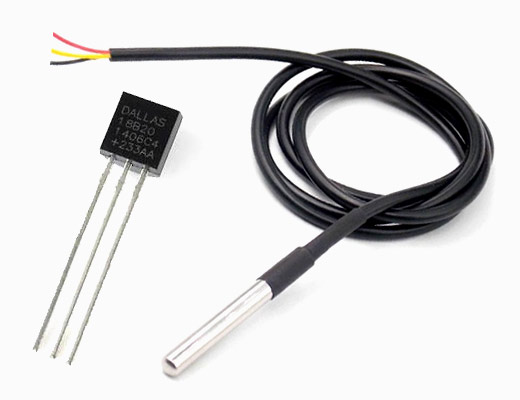
\includegraphics[width=0.3\textwidth]{./pics/TempSensBild.jpeg}
    \caption{TemperaturSensor}
    \label{fig:TemperaturSensor}
\end{figure}




\newpage
\subsection*{pH-Sensor:}
Der E-201-C ist ein pH-Sensor, der zur Messung des pH-Werts von Flüssigkeiten und Lösungen verwendet wird. Es ist ein elektrochemischer Sensor, der durch die Messung der Spannung zwischen einer pH-sensitiven Elektrode und einer Referenzelektrode arbeitet.
Der E-201-C pH-Sensor besteht aus einer pH-sensitiven Glaselektrode und einer Referenzelektrode. Die pH-sensible Glaselektrode besteht aus einem dünnen Glasrohr, das mit einer pH-sensitiven Membran beschichtet ist. Die Referenzelektrode besteht aus einem inneren Leitungsstab, der von einem keramischen Elektrolyten umgeben ist, der mit einer Referenzlösung gefüllt ist. Der Sensor wird über eine BNC-Buchse an ein Messgerät angeschlossen.
Der E-201-C bietet eine hohe Genauigkeit und Empfindlichkeit mit einer Auflösung von 0,01 pH-Einheiten und einer Genauigkeit von ±0,1 pH-Einheiten im Temperaturbereich von 0 bis 80°C. Der Sensor bietet auch eine schnelle Reaktionszeit, wodurch Messungen in Echtzeit durchgeführt werden können.
Ein weiterer Vorteil des E-201-C pH-Sensors ist seine hohe Stabilität und Haltbarkeit. Die pH-sensible Membran ist chemisch inert und widerstandsfähig gegenüber Korrosion und Abnutzung. Dies gewährleistet eine lange Lebensdauer des Sensors und eine genaue Messung über einen längeren Zeitraum.
Der E-201-C pH-Sensor wird in einer Vielzahl von Anwendungen eingesetzt, darunter in der chemischen Industrie, der Lebensmittelindustrie, der Umweltüberwachung und der pharmazeutischen Industrie. Es ist ein wichtiger Sensor zur Messung des pH-Werts in Lösungen und Flüssigkeiten, um sicherzustellen, dass sie den erforderlichen Spezifikationen entsprechen. 
\newline
Datasheet: \url{https://www.e-gizmo.net/oc/kits%20documents/PH%20Sensor%20E-201-C/PH%20Sensor%20E-201-C.pdf}

\begin{figure}[b]
    \centering
    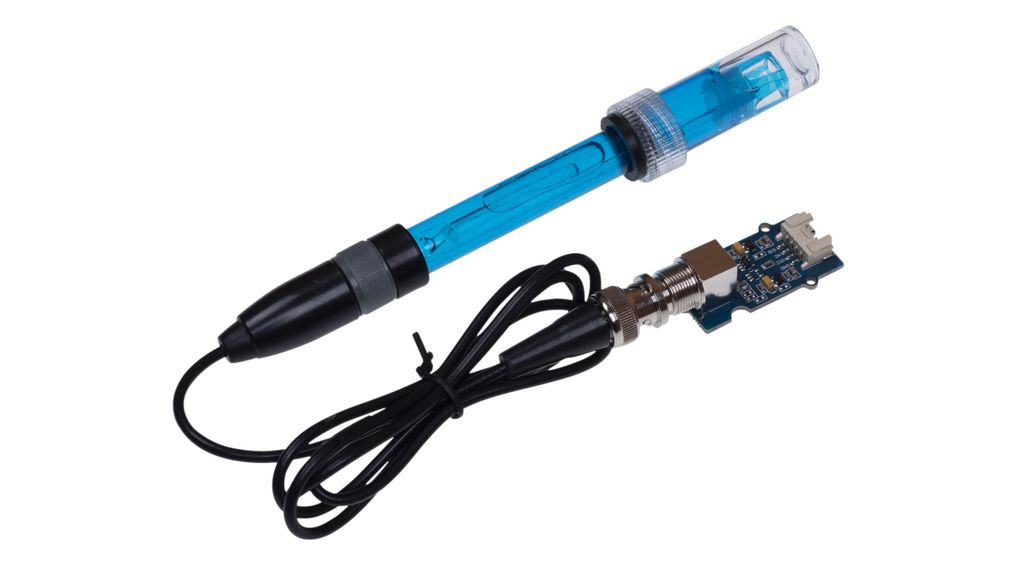
\includegraphics[width=0.7\textwidth]{./pics/pHSensorBild.jpeg}
    \caption{Ph-Sensor}
    \label{fig:TTGO-ESP32}
\end{figure}

\newpage
\subsection*{NTU-Sensor|Trübungs-Sensor:}
Das TS-300B Trübungssensor-Modul ist ein Qualitäts-Trübungssensor, der zur Messung der Trübung von Flüssigkeiten verwendet wird. 
Es ist ein optischer Sensor, der durch Messung des Streulichts arbeitet, das von Verunreinigungen in der Flüssigkeit reflektiert wird.
Das TS-300B Trübungssensor-Modul besteht aus einem Gehäuse, das einen Infrarot-LED-Lichtquelle und einen Phototransistor-Sensor enthält. 
Der LED-Lichtquelle strahlt Infrarotlicht aus, das von den Verunreinigungen in der Flüssigkeit gestreut wird. Der Phototransistor-Sensor misst dann das Streulicht, um die Trübung der Flüssigkeit zu bestimmen. 
Dieser Trübungssensor bietet eine hohe Empfindlichkeit und Genauigkeit mit einer Messauflösung von bis zu 0,1 NTU (Nephelometric Turbidity Unit) und einer Messgenauigkeit von ±5 Prozent im Bereich von 0 bis 1000 NTU. 
Der Sensor bietet auch eine schnelle Reaktionszeit und kann Trübungen in Echtzeit messen. Der Sensor kann über einen einfachen Analogausgang an ein Messgerät oder einen Mikrocontroller angeschlossen werden. Es ist auch einfach zu installieren und zu warten, da es keine beweglichen Teile hat und daher eine geringe Wartung erfordert. 
Der TS-300B Trübungssensor wird in einer Vielzahl von Anwendungen eingesetzt, darunter in der Wasseraufbereitung, der Abwasserbehandlung, der Lebensmittel- und Getränkeindustrie und der Umweltüberwachung. Es ist ein wichtiger Sensor zur Messung der Wasserqualität und zur Überwachung von Prozessen, die von der Trübung der Flüssigkeit abhängen. 


Datasheet: \url{https://de.aliexpress.com/item/4000321791231.html}

\begin{figure}[b]
    \centering
    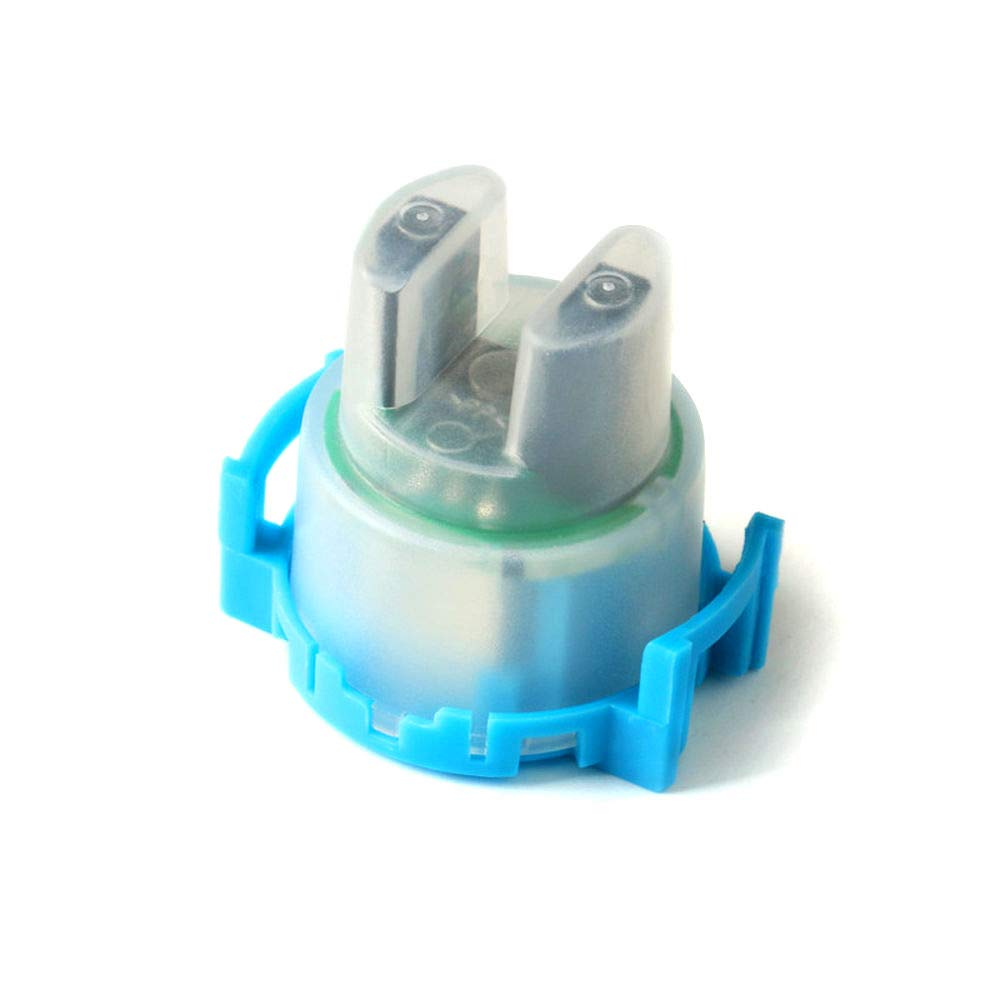
\includegraphics[width=0.4\textwidth]{./pics/ntuSensorBild.jpeg}
    \caption{NTU-Sensor}
    \label{fig:NTU-Sensor}
\end{figure}



\newpage
\subsection*{Gyroskop/Beschleunigunssensor:}
Der SEN-MPU6050 ist ein Kombinationssensor, der sowohl einen Gyroskop- als auch einen Beschleunigungssensor enthält. 
Diese beiden Sensoren arbeiten zusammen, um die Bewegungen und Orientierungen eines Objekts in der Raumebene zu messen. 
Der Sensor misst die Winkelgeschwindigkeit eines Objekts um seine drei Achsen (x, y, z). Der Sensor erfasst dabei die Änderungen der Rotationsgeschwindigkeit, die durch die Drehung des Objekts verursacht werden. 
Der Beschleunigungssensor hingegen misst die Beschleunigung des Objekts in jeder der drei Achsen (x, y, z). 
Der Sensor erfasst dabei die Änderungen der Geschwindigkeit, die durch eine Beschleunigung oder Verzögerung des Objekts verursacht werden. 
Der SEN-MPU6050 bietet eine hohe Genauigkeit und Empfindlichkeit mit einer Auflösung von bis zu 16 Bit für beide Sensoren. 
Der Gyroskop-Sensor bietet eine hohe Genauigkeit mit einer maximalen Abweichung von nur 3,8 Grad pro Sekunde, während der Beschleunigungssensor eine Genauigkeit von ±2 g bietet. 
Der Sensor bietet auch eine schnelle Reaktionszeit mit einer Abtastrate von bis zu 1 kHz für den Gyroskop-Sensor und bis zu 4 kHz für den Beschleunigungssensor. 
Der SEN-MPU6050 wird in einer Vielzahl von Anwendungen eingesetzt, darunter in der Robotik, der Luft- und Raumfahrt, der Drohnensteuerung, der Navigation, der virtuellen Realität und der Spieleentwicklung. 
Es ist ein wichtiger Sensor zur Messung der Bewegung und Orientierung von Objekten in der Raumebene. 
\newline
Datasheet: \url{https://joy-it.net/de/products/SEN-MPU6050} 

\begin{figure}[b]
    \centering
    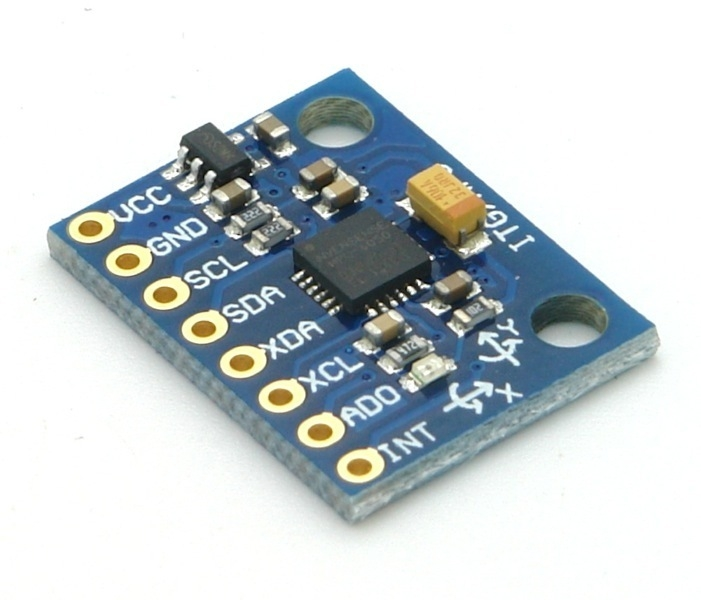
\includegraphics[width=0.4\textwidth]{./pics/BeschlSensorBild.jpeg}
    \caption{Beschleunigungssensor}
    \label{fig:Beschleunigungssensor}
\end{figure}



